%% intro.tex
%% Copyright 2013 M. J. Gidden

% This program can redistributed and/or modified under the terms
% of the LaTeX Project Public License Distributed from CTAN
% archives in directory macros/latex/base/lppl.txt; either
% version 1 of the License, or (at your option) any later version.

The 2013 Nuclear Engineering Student Delegation (NESD) was held in Washington,
D.C., on July 6-12, 2013. Formed in 1994 to reinstate funding for research
reactors, the delegation continues to express the views of the student
population on nuclear science and engineering education. The delegation is
independently selected and organized with funding and support provided by the
Nuclear Energy Institute (NEI) and the American Nuclear Society (ANS). This
year's delegation was comprised of sixteen students from twelve universities
across the country. Pictures of the delegates are shown below in
Figure~\ref{fig:delegates} and biographies for each delegate follow.

\begin{figure}[h]
\centering
\begin{subfigure}{.5 \textwidth}
  \centering
  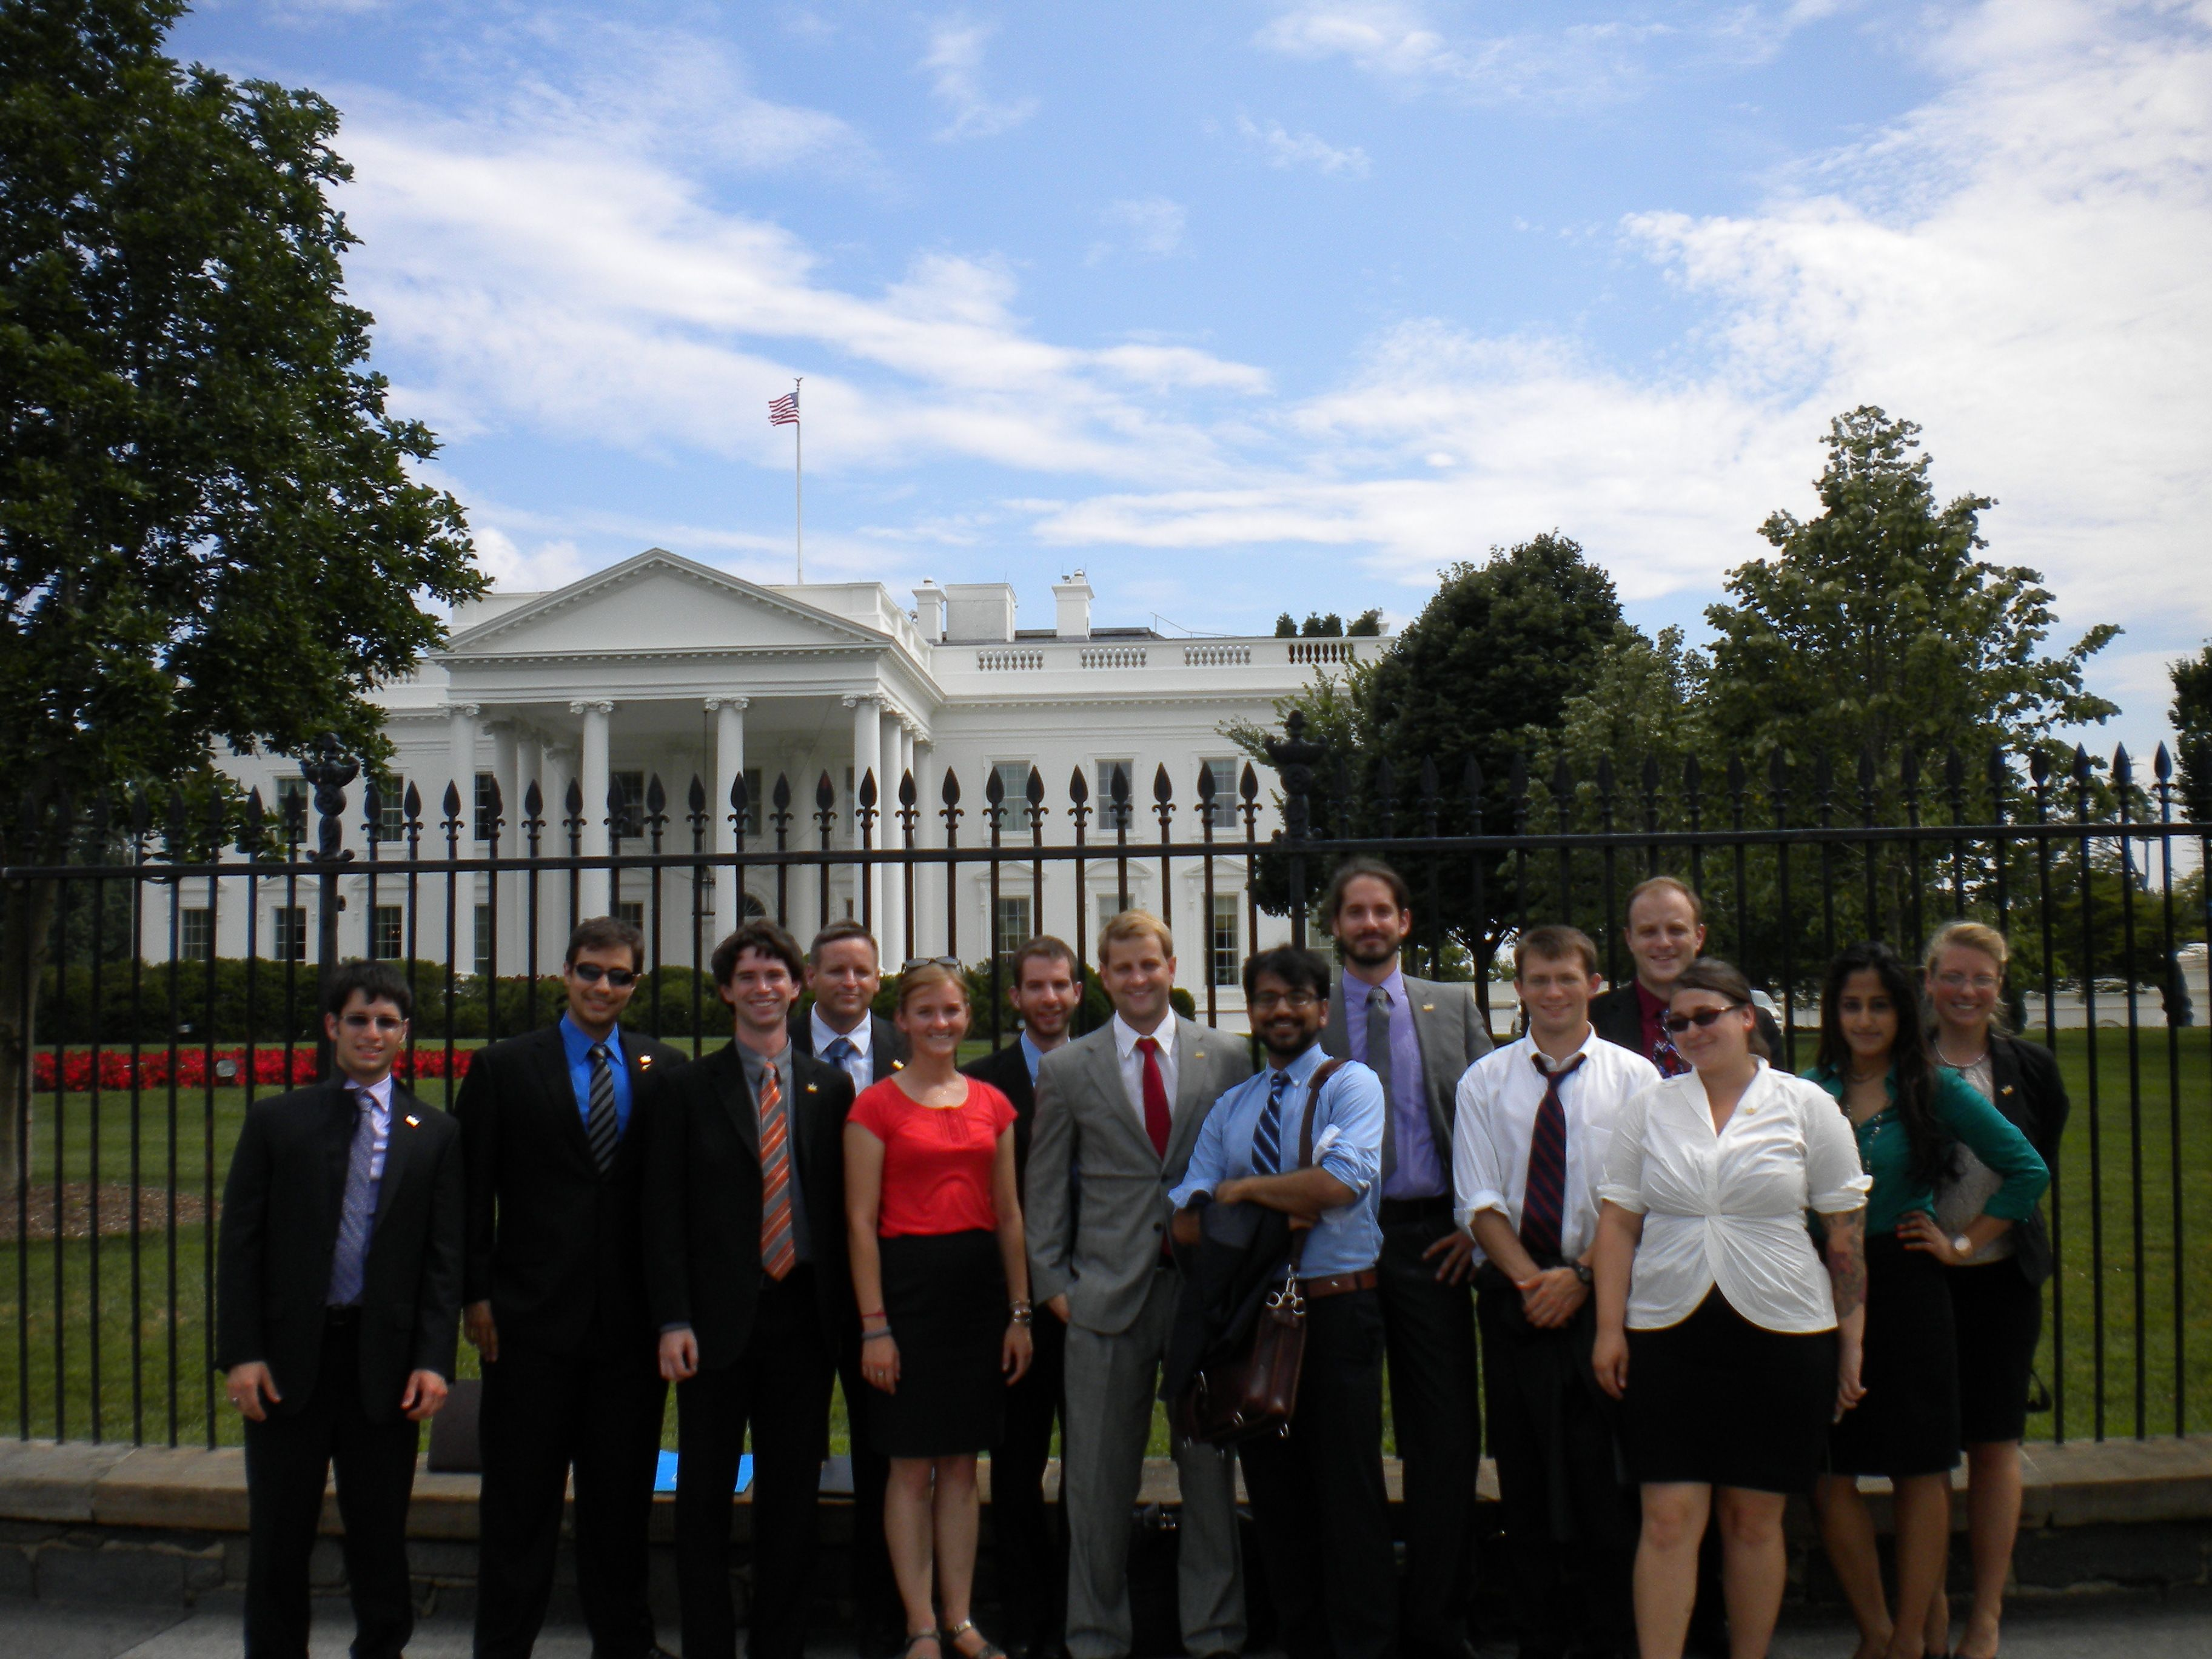
\includegraphics[width=.95 \linewidth]{NESD_WH.jpg}
  \label{fig:whitehouse}
\end{subfigure}%
\begin{subfigure}{.5\textwidth}
  \centering
  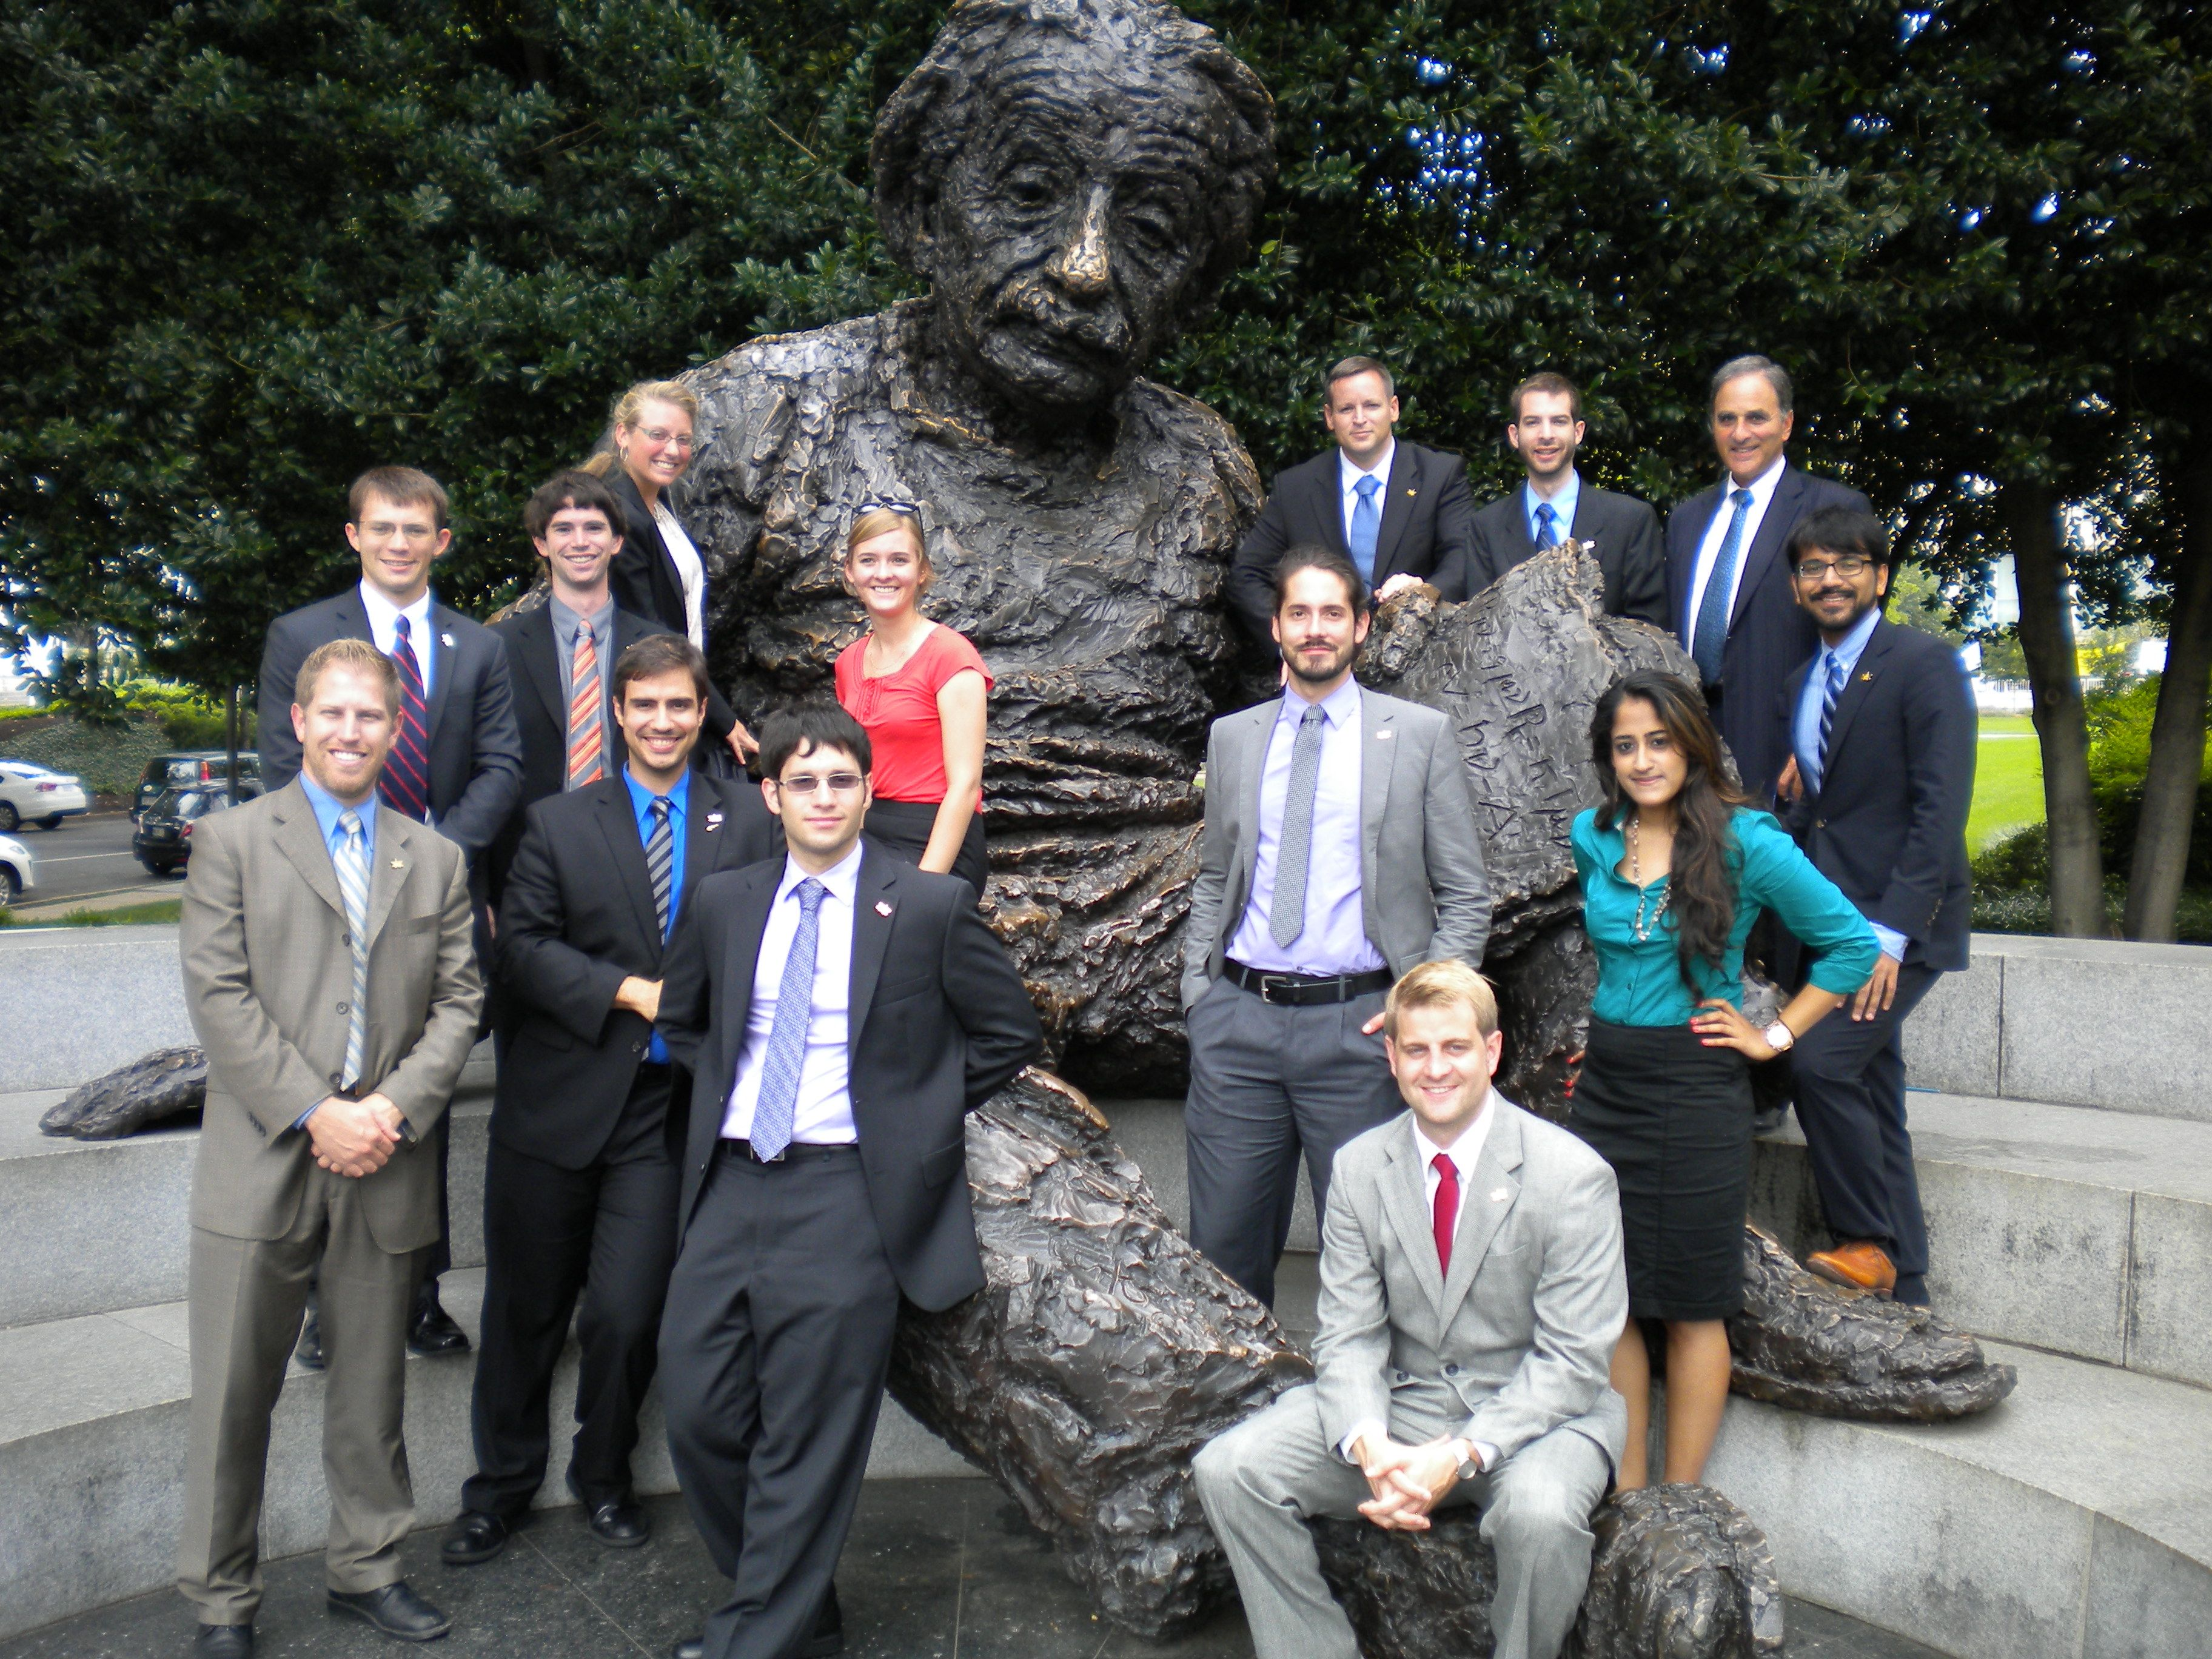
\includegraphics[width=.95 \linewidth]{NESD_Ein.jpg}
  \label{fig:einstein}
\end{subfigure}
\caption{The Delegation at the White House and National Academies}
\label{fig:delegates}
\end{figure}

\subsubsection*{Matthew Gidden, University of Wisconsin - Madison (Chair)}

Matthew is a Ph.D. graduate student at the University of Wisconsin - Madison
studying nuclear engineering and energy policy. He previously attended Texas
A\&M University where he received a B.S. in nuclear engineering. Matthew
currently works in the Fuel Cycle Research Group at UW - Madison under Professor
Paul Wilson. His research interest is primarily fuel-cycle simulation and
analysis and related policy topics, such as used-fuel recycling, long-term fuel
storage, and nuclear nonproliferation.

Matthew is an active member of the American Nuclear Society, serving as the 2008
Student Conference Co-Chair as well as participating in the governance of ANS at
the national level. He has previously held internship positions at both Oak
Ridge National Laboratory working on the detection of illicit radioactive
materials and Pacific Northwest National Laboratory working on automated
verification techniques. He has also had the opportunity to work for AREVA in
Paris, France on both the transportation of used nuclear fuel as well as nuclear
reactor accident analysis.

\subsubsection*{Mark Reed, Massachusetts Institute of Technology (Co-Vice Chair)}

Mark has received his S.B. degree in Physics as well as his S.B. and
S.M. degrees in Nuclear Science and Engineering from MIT, and he is currently a
Ph.D. candidate in Nuclear Science and Engineering at MIT. His past research
includes magnetic confinement fusion and its application as a neutron source in
fission-fusion hybrid systems, enhanced fission yield modeling techniques, and
strategic plant siting in the context of seismic history. His current doctoral
research focuses on the neutronic effects of geometric distortions in fast
reactors.

He has performed reactor modeling at TerraPower and risk assessment for the
Yucca Mountain Nuclear Waste Repository at the U.S. Nuclear Regulatory
Commission. In his pre-nuclear life, he was an engineering project management
intern for the iPhone 3G at Apple and a research assistant at the Princeton
University Department of Astrophysical Sciences. Passionate about nuclear
policy, he has published a series of six articles on the history of nuclear
technology, served as a speechwriter for an elected official, and conceived the
2013 American Nuclear Society Student Conference theme ``Public Image of the
Nuclear Engineer''. In his spare time, he pursues his affinities for hiking,
making random iPhone applications, and composing awkward third-person
autobiographies.

\subsubsection*{Nicholas Thompson, Rensselaer Polytechnic Institute (Co-Vice Chair)}

Nicholas is a Ph.D. student at Rensselaer Polytechnic Institute (RPI) studying
Nuclear Engineering and Science. He graduated RPI in 2011 with a B.S. and an
M.Eng. in Nuclear Engineering. He has previously held two summer internships at
Knolls Atomic Power Laboratory, and from 2010 to 2011, was an undergraduate
researcher at the Gaerttner Linear Accelerator Center (LINAC) at RPI.

Nick's current research focuses on using a Lead Slowing-Down Spectrometer
(LSDS)for measuring various nuclear data. In particular, two of the projects he
is working on are to make capture cross section measurements and fission
fragment distribution measurements, both with the LINAC and RPI LSDS. While
working as an undergraduate researcher, Nick helped research and perform
experiments with the RPI LSDS to assay plutonium and uranium with the goal of
nondestructively assaying spent fuel. Nick was selected as a winner of the
Innovations in Fuel Cycle Research Award and presented this research at the 2011
American Nuclear Society (ANS) Winter Conference. He was also the President of
the RPI ANS section from 2012-2013. Nick was also an NESD delegate in 2012, and
one of the Co-Vice Chairs in 2013. Some of Nick's research interests include
nuclear data, reactor design, accelerator technologies and applications, and
nuclear energy policy. Nick is an avid skier, enjoys playing billiards, and
believes that cheap, clean, reliable, safe nuclear power can help the economy
and the environment.

\subsubsection*{Shelly Arreguin, University of Washington}

Shelly is a Materials Science and Engineering (MSE) Ph.D. student at the
University of Washington in Seattle (UW). She obtained a M.S. in MSE from the UW
and B.S. degrees in Chemistry from the University of Colorado at Boulder
(CU) and Ecology, Evolution \& Conservation Biology at UW. Her primary research
interest involves investigating the relationship of processing and properties of
materials and their performance under extreme conditions (nuclear, high
temperature, accident scenarios, etc.).

Shelly has worked extensively on developing unique processing routes from
preceramic polymers to test their capabilities in various energy applications
such as: catalysts for fuel cells (CU), hydrogen storage (National Renewable
Energy Laboratory), waste-to-energy incinerators (UW) and now high temperature
nuclear environments (UW). Previously, Shelly held an appointment at the Pacific
Northwest National Laboratory (PNNL) as a Mickey Leland Energy Fellow where she
designed chalcohalide glasses for the storage of nuclear waste streams with
increased halide content. Currently, she is at PNNL exploring the
microstructural evolution of irradiated porous and dense polymer derived SiC
ceramics for her Ph.D. thesis. When not in the lab, Shelly enjoys: cave
exploration, studying extremophiles and their associated geology, NASA's Kepler
Mission, understanding the role of bio-indicators of environmental
contamination, mushroom hunting, SCUBA and public outreach, exposing myths
vs. realities in nuclear science and technology.

\subsubsection*{Sam Brinton, Massachusetts Institute of Technology}

Samuel is completing a double M.S. program at Massachusetts Institute of
Technology in Nuclear Engineering and the Technology and Policy Program. He is a
graduate from Kansas State University with a B.S. in Mechanical and Nuclear
Engineering and a B.A. in Vocal Music Performance and a minor in Chinese
Language. His research interests are concentrated on nuclear fuel cycle system
analysis with subtopics of interest including fuel cycle economics and dry cask
storage analysis.

Samuel has had internships at the Argonne National Laboratory, Idaho National
Laboratory, and Dow Chemical Company in various projects relating to nuclear
engineering and systems analysis. He is a strong activist in a variety of civil
rights and nonproliferation issues and finds that only with a constant
interaction with our legislative representatives can we hope to make true and
lasting impacts on policy. In his spare time Samuel enjoys running, singing with
choirs and opera companies, and cheering for the K-State Wildcats and MIT
Engineers.

\subsubsection*{Lane Carasik, Texas A\&M University}

Lane is a graduate student at Texas A\&M University studying nuclear and
mechanical engineering. He recently graduated with his B.S. in Nuclear
Engineering from the University of Tennessee, Knoxville where he conducted
nuclear thermal hydraulics research under Dr. Arthur Ruggles. Lane will be a
part of the Nuclear Power Engineering Research group at TAMU under Dr. Yassin
Hassan. His research interests are in nuclear reactor thermal hydraulics and
methods development for computational fluid dynamics and heat transfer.

Lane is an active member of the American Nuclear Society and American Society of
Mechanical Engineers. Lane is currently the Vice Chair of the ANS Student
Section Committee and serving on the Executive Committee for the Thermal
Hydraulics Division. Lane has previously been the Chair of the UTK ANS Student
Section and the student chair for PHYSOR 2012. Lane has had previous internships
at Westinghouse Electric Company and Tennessee Valley Authority working on
reactor coolant systems. At Westinghouse Electric Company, Lane worked on steady
state and transient analysis for Electricite de France reactor coolant system
components and CFD method development.

\subsubsection*{Andrew Cartas, University of Florida}

Andrew is a Ph.D. student at the University of Florida studying Nuclear
Engineering where he obtained his B.S. in Nuclear Engineering in 2011. His
current research focus is on nuclear fuel fabrication, utilizing depleted
Uranium, and material performance under irradiation. Andrew has also focused his
research efforts on Silicon Carbide as a fuel additive and matrix material for
UO2.

Andrew has been heavily involved in the University of Florida ANS student
section having served two years as treasurer and is the outgoing section
president. During the summer of 2011, he was selected to be the student chair
for the 2011 ANS National Conference in Hollywood, FL. He is currently serving
on ANS National Subcommittee for Disbursement of ANS Travel Funds to
Students. Andrew has interned at Argonne National Lab and participated in the
Nondestructive Assay Applications for International Safeguards program held at
Oak Ridge National Lab.

\subsubsection*{Erin Dughie, University of New Mexico}

Erin is a Ph.D. graduate student at the University of New Mexico studying nuclear
engineering. She recently graduated with her undergraduate and M.S. degrees
from the University of Michigan in 2011 and 2012, respectively. Her research
interests include radiation detection and measurements. In the past she has
worked on detection techniques for nonproliferation, and semiconductor
devices. Her current work focuses on the detection of dark matter.

Erin is an active member of IEEE and the American Nuclear Society. She has
previously held internships at Los Alamos National Laboratory working on MCNPX
code development, and space nuclear power. In her free time, Erin is involved in
outreach activities at the local science museum. She also works with several
programs at the University of New Mexico that facilitate K-12 science and
technology activities.

\subsubsection*{Tom Grimes, Purdue University}

Tom has received a B.S. degree from Purdue University in Nuclear Engineering and
is currently a Ph.D. graduate student at Purdue University studying Nuclear
Engineering as well as an MBA student with a focus on Entrepreneurship. Tom
currently works in the Metastable Fluid and Advanced Research Lab under
Professor Rusi Taleyarkhan. He is currently funded through the National Science
Foundation Graduate Research Fellow Program. His research interests include
nuclear non-proliferation, fluid dynamics, radiation transport, acoustics, and
materials (he holds an international patent for PLA-based coatings).

Tom's current doctoral research focuses on developing a fundamental physics
model to describe the operation of Metastable Fluid Detectors (with wider
application toward general cavitation studies e.g. making quieter submarines or
faster jet planes). His first brush with nuclear policymaking came while
evaluating Metastable Fluid Detectors for application in Radiation Portal
Monitors. Since then he has maintained a strong interest in border security and
non-proliferation policy.

\subsubsection*{Tommy Holschuh, Oregon State University}

Tommy is currently pursuing a M.S. degree in nuclear engineering at Oregon
State University in Corvallis, OR. He received a B.S. in nuclear engineering
from OSU in 2013.

Tommy began performing research for Sandia National Laboratories in 2007 and
Oregon State University in 2010. His previous research areas include
magnetically-confined fusion, supercritical CO2 Brayton cycle systems,
irradiation experiments, and advanced diagnostics for the U.S. research reactor
fuel conversion program. Additionally, he is involved in OSU's student chapter
of the American Nuclear Society, in which he leads outreach programs for Boy
Scouts and other local youth groups.

For his graduate work, he will be involved in the High Temperature Test
Facility, a scaled gas reactor facility, as a research assistant under Dr. Brian
Woods. Tommy enjoys living in Oregon and likes trail running, rock climbing, and
soccer.

\subsubsection*{Anagha Iyengar, University of Tenneessee}

Anagha Iyengar is a Ph.D. student in the Nuclear Engineering department at the
University of Tennessee, Knoxville. She received her B.S. in Nuclear Engineering
from the University of California, Berkeley in 2012. Her research interests lie
in nuclear security, nonproliferation technologies, international relations and
energy policy. She is working on her graduate research in collaboration with Oak
Ridge National Laboratories under Dr. Jason Hayward, and is a part of the
Nuclear Materials Detection and Characterization group. Her current research
focuses on developing a passive mobile neutron detection system for
nonproliferation and security applications.

Anagha is an active member of the American Nuclear Society (ANS), Institute for
Electrical and Electronics Engineers (IEEE), and the Institute of Nuclear
Materials Management (INMM). In the past, she has had internships working on
developing and characterizing novel detection technologies at UC Berkeley,
Lawrence Berkeley National Laboratories, Lawrence Livermore National
Laboratories (Next Generation Safeguards Initiative Intern), and Sandia National
Laboratories. She is passionate about outreach efforts in local communities and
schools to advocate and encourage STEM education. She also writes for the
Nuclear Literacy Project to help dispel myths about the nuclear industry. In her
spare time, Anagha enjoys traveling, hiking, and baking.

\subsubsection*{Buck O'Day, Massachusetts Institute of Technology}

Buck is a Ph.D. Graduate student at the Massachusetts Institute of Technology
studying Nuclear Science and Engineering. He previously attended the Air Force
Institute of Technology where he earned a M.S. in Nuclear Engineering, the
University of Maryland University College where he earned a Master of
International Management, and the United States Military Academy where he earned
a B.S. in Civil Engineering. He currently studies nuclear materials detection
under MIT Senior Research Scientist Dr. Dick Lanza. His research interests
include detection of nuclear materials, nuclear policy \& security, radiation
effects, and nuclear nonproliferation.

\subsubsection*{Katia Paramonova, Massachusetts Institute of Technology}

Ekaterina (Katia) Paramonova is a Masters graduate student at the Massachusetts
Institute of Technology (MIT) studying Nuclear Science and Engineering
(NSE). She completed her B.S. at MIT with a major in NSE and a minor in Public
Policy. Katia is working on experimental materials research on mitigating the
deposition of CRUD with Professor Michael Short. She plans on going to France
for her Ph.D. in nuclear engineering to get a third view on the industry in
addition to her US and Russian perspectives. After completing her studies, Katia
then wants to work in the industry or at a think tank for some time before
moving on to international energy policy, with a focus on nuclear energy.

Katia is an active member of the American Nuclear Society (ANS). She is the
2013-2014 co-President of the MIT ANS section and was a co-Chair for the 2013
ANS Student Conference held at MIT. She has interned at Westinghouse, worked on
various research projects at MIT including MCNP-Serpent benchmarking work,
copper 63 and 65 capture cross section measurements, public perception of
nuclear systems modeling, and a summer project at the Harvard Managing the Atom
Center on nuclear materials in Russia. She also takes delegations of students
from MIT to Russia in the summers for conferences, assists in the Russian
SkolTech Institute nuclear center development, and is working on establishing a
student exchange program between MIT and Russia universities. Her goal is to
bring together nations as well as policy and technical experts together to help
innovation flourish.

\subsubsection*{Vishal Patel, Texas A\&M University}

Vishal is a Ph.D. graduate student at Texas A\&M University studying Nuclear
Engineering. He has received an M.S. in Nuclear Engineering from Texas A\&M and
a B.S. in Physics from The University of Texas. Vishal currently works in the
Advanced Energy Technologies group under Professor Pavel Tsvetkov. His research
interests include advanced reactor concepts and reactor control.

Vishal previously performed undergraduate research in neutron activation
analysis and was an undergraduate TA in a radiation detection lab at UT. He has
done summer work at the Center for Space Nuclear Research at the INL developing
a nuclear electric propulsion spacecraft. Outside of his academic pursuits,
Vishal enjoys weightlifting, cooking, and searching for the perfect cup of
coffee.

\subsubsection*{Jeremy Pearson, University of California - Irvine}

Jeremy is a Ph.D. graduate student at the University of California - Irvine
studying chemical engineering and used nuclear fuel recycling. He previously
attended Brigham Young University where he received a B.S. in chemical
engineering. Jeremy currently works in the Nuclear Research Group at UC Irvine
under Professor Mikael Nilsson. His research interest focuses on understanding
the sensitivity of solvent extraction processes to radiolysis in an effort to
create more robust, efficient, and economical processes which can be adopted in
a future fuel cycle that includes recycling and advanced reactor technologies.

Jeremy is an active member of the American Nuclear Society, serving on the
Education and Public Outreach committees in the San Diego ANS Local Section. In
this capacity he has given lectures on nuclear science and technology at local
high schools and worked to promote awareness of nuclear energy and technology,
especially during the NRC's evaluation for restart of the local San Onofre
Nuclear Generating Station, by organizing and hosting screenings of Switch and
Pandora's Promise at UC Irvine with their respective directors. Jeremy has also
participated with colleagues representing UCI in D.C. at the DOE's Better
Building's Case Competition presenting energy efficiency solutions to the
government's real estate portfolio managed by the GSA. In his spare time Jeremy
enjoys playing guitar, wake surfing, and playing soccer and dirt biking with his
family.

\subsubsection*{Ben Reinke, The Ohio State University}

Benjamin Reinke is a Ph.D. student at the Ohio State University studying Nuclear
Engineering. He graduated from OSU with a B.S. in Physics and French and Honors
and Research Distinction in 2010. While an undergraduate, he worked in a High
Energy Density Physics laser research laboratory.

Ben is a NASA Space Technology Research Fellow. His current research focuses on
experimental and simulations for cryogenic irradiation damage
tests. Specifically Ben is establishing a cryogenic irradiation facility at the
Ohio State University Research Reactor for completing in situ damage tests on
semiconductor materials and optical fibers. Ben also works with a Material
Science professor to simulate the radiation damage in these experiments and
develop a mulit-scale model of defect annealing. Earlier in his graduate
studies, Ben worked on a Department of Energy Nuclear Engineering Program to
develop a high temperature alpha particle detector with 4H-SiC. Ben also spends
time as the president of the OSU student chapter of the American Nuclear Society
and serving as the graduate/professional student member of the OSU Board of
Trustees.
